% !TeX root = ../main.tex
\section{Результаты имитационного моделирования}

Моделирование устройства обнаружения сигналов со стабилизацией уровня ложных тревог с оценкой меньшего среднего значения (ОБН с СУЛТ-МСЗ) выполнено в среде MATLAB для параметров варианта ($q = 20\text{ дБ}$, ОПШ $= 15;\; 35\text{ дБ}$, $P_{\text{лт}} = 10^{-5}$, $N = 16$, $N_G = 1$, $N_M = 3$).

\subsection{Поведение порога обнаружения в гомогенных условиях}

На первом этапе исследовано поведение адаптивного порога при обнаружении одиночной точечной цели (500-й отсчет дальности) на фоне однородного собственного шума приемника. Результат моделирования представлен на рисунке~\ref{fig:he_tb}.

\begin{figure}[H]
    \centering
    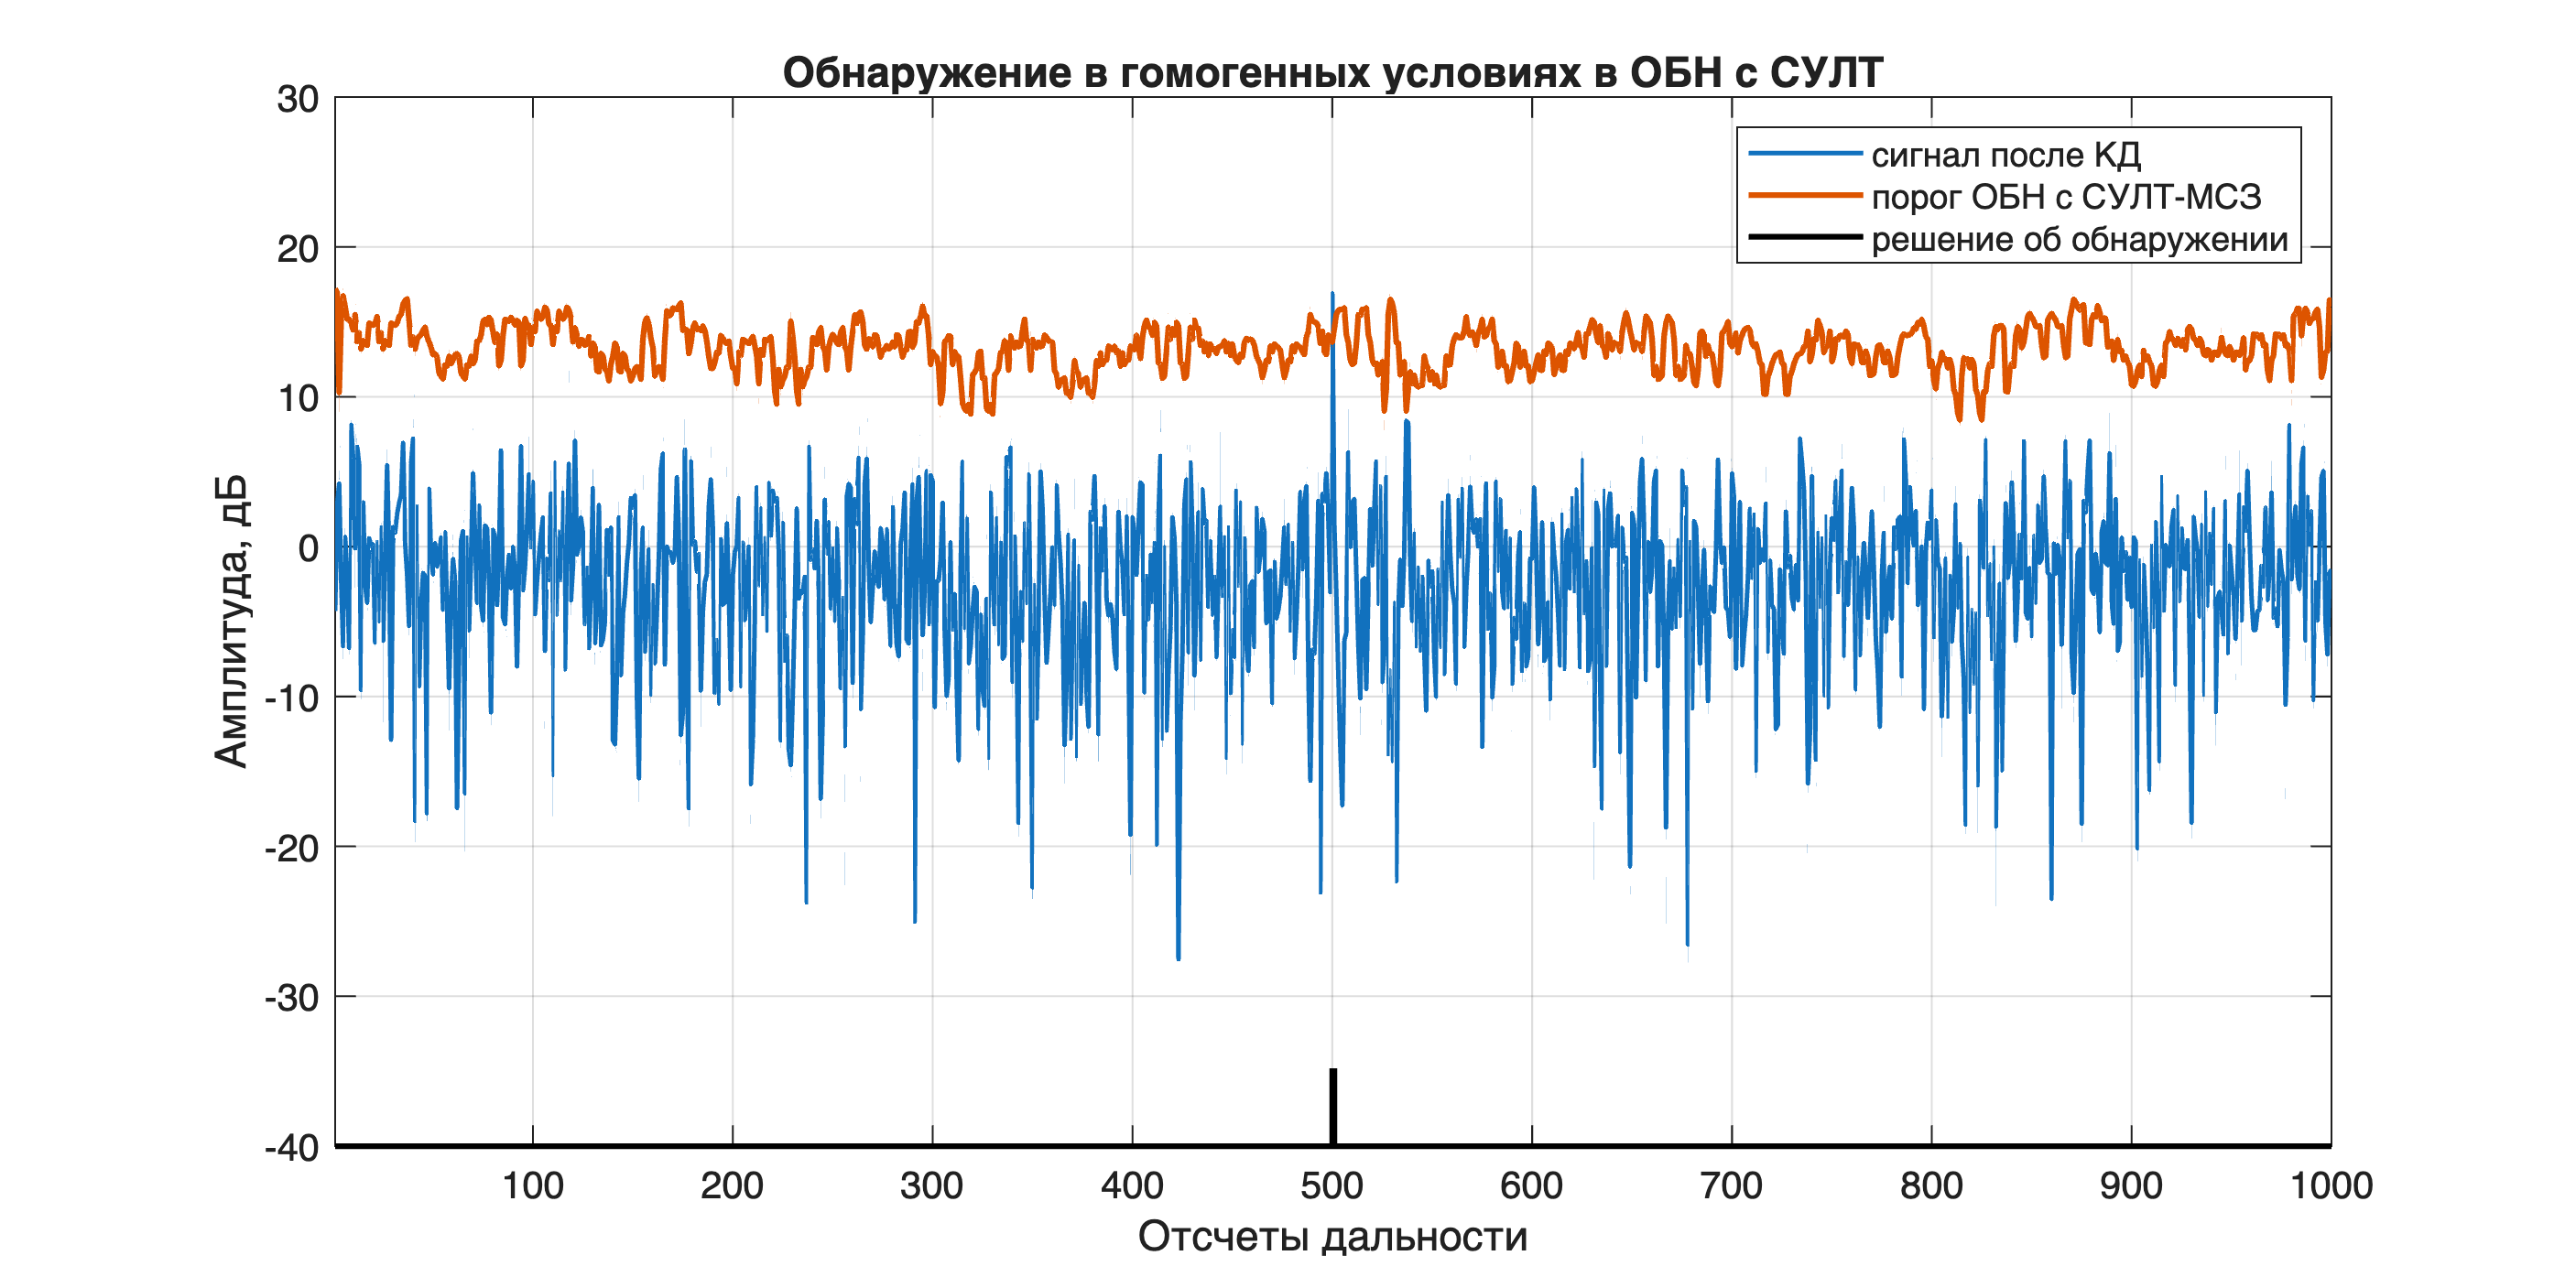
\includegraphics[width=0.85\textwidth]{export_figs/fig_he_tb.png}
    \caption{Обнаружение цели в гомогенных условиях в ОБН с СУЛТ-МСЗ}
    \label{fig:he_tb}
\end{figure}

Из временной диаграммы видно, что на всем интервале наблюдения ($1000$ отсчетов дальности) адаптивный порог обнаружителя отслеживает средний уровень флуктуаций шума и удерживается в пределах $10\dots16\text{ дБ}$. В окрестности 500-го отсчета благодаря наличию защитных ячеек ($N_G = 1$) энергия полезного эхо-сигнала не попадает в обучающую выборку, поэтому завышения порога не происходит и цель уверенно обнаруживается без возникновения ложных срабатываний на остальной дистанции.

\subsection{Поведение порога обнаружения на границе помех}

На втором этапе исследовано поведение адаптивного порога в гетерогенных условиях — при ступенчатом перепаде мощности помехи с уровня ОПШ $= 15\text{ дБ}$ до уровня ОПШ $= 35\text{ дБ}$ на $500$-м отсчете дальности. Полезный сигнал от цели расположен в области меньшей помехи на $450$-м отсчете. Результат моделирования представлен на рисунке~\ref{fig:cwe_tb}.

\begin{figure}[H]
    \centering
    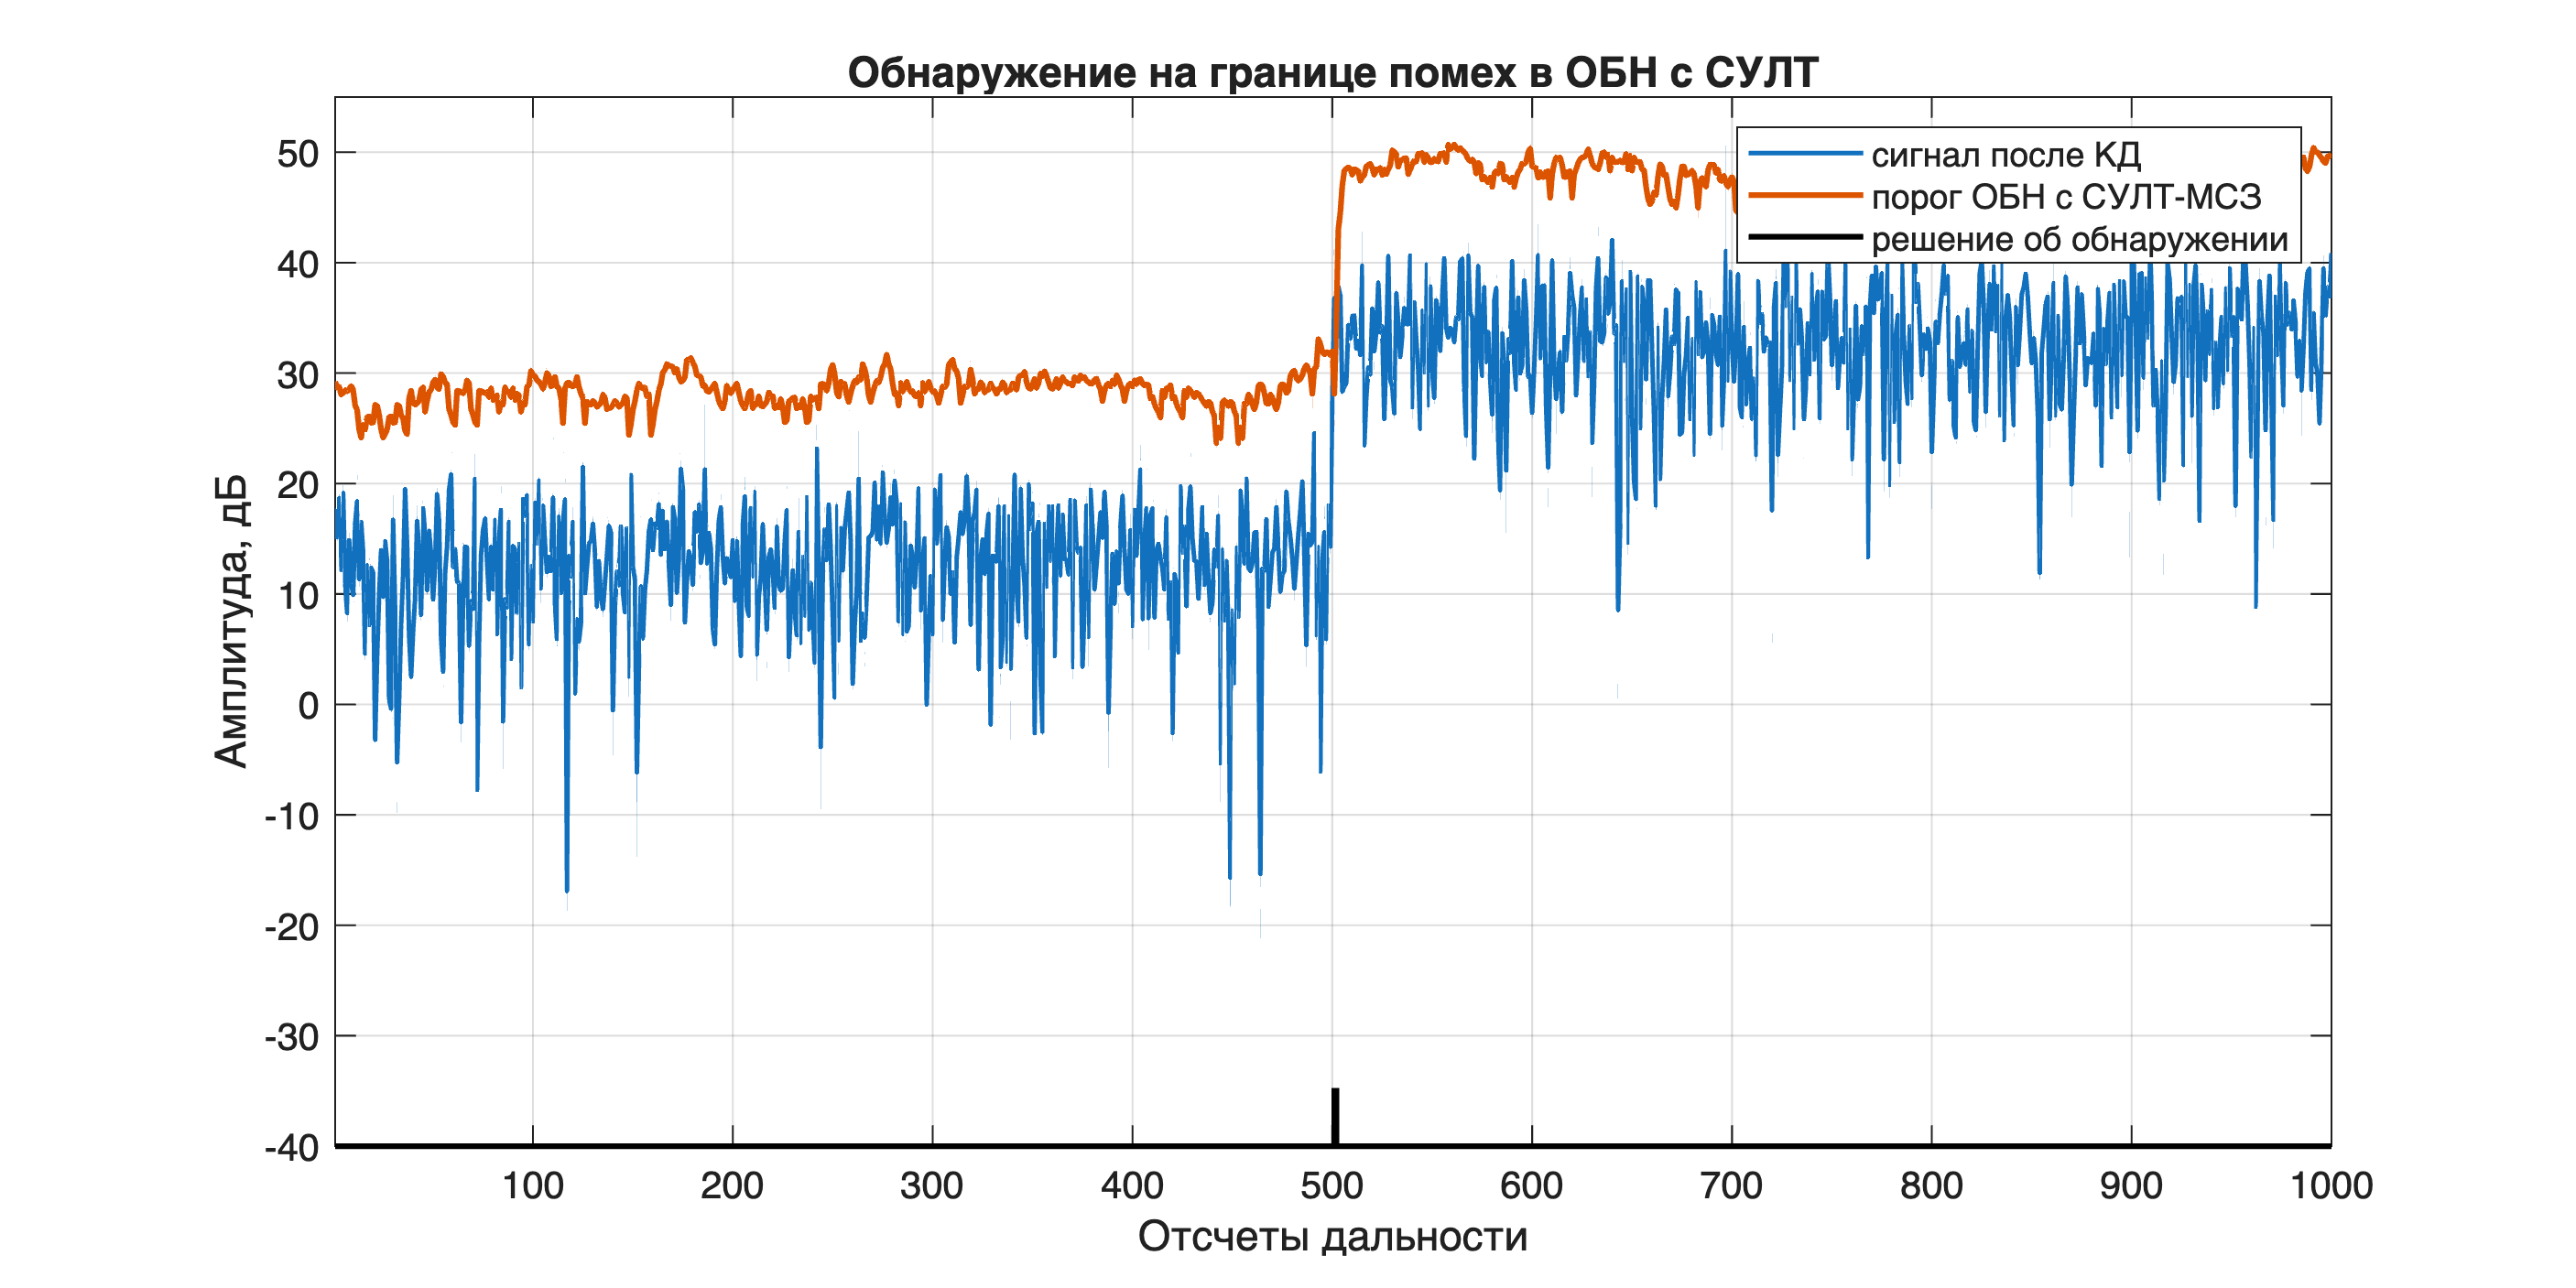
\includegraphics[width=0.85\textwidth]{export_figs/fig_cwe_tb.png}
    \caption{Обнаружение на границе помех в ОБН с СУЛТ-МСЗ}
    \label{fig:cwe_tb}
\end{figure}

Анализ диаграммы демонстрирует ключевую особенность алгоритма МСЗ на границе раздела помех. Когда тестируемый отсчет переходит в область интенсивной помехи (сразу после $500$-го отсчета), отстающая часть скользящего окна все еще располагается в области с низким уровнем помехи ($15\text{ дБ}$). Поскольку обнаружитель выбирает минимум из двух полуокон, пороговый уровень не успевает своевременно вырасти до требуемых $\approx 48\dots50\text{ дБ}$. Это приводит к занижению порога непосредственно за границей скачка помехи и возникновению ложного обнаружения в районе $500$-го отсчета. При этом в данной случайной реализации флуктуаций амплитуда полезного сигнала на $450$-м отсчете не превысила текущий порог ($\approx 26\text{ дБ}$).

\subsection{Поведение порога обнаружения при наличии близкорасположенных целей}

На третьем этапе исследована работа обнаружителя с СУЛТ-МСЗ в гетерогенных условиях при наличии группы из близкорасположенных целей (основная и $N_M = 3$ мешающих цели на отсчетах дальности $490$, $500$, $510$ и $520$). Результат моделирования представлен на рисунке~\ref{fig:hmte_tb}.

\begin{figure}[H]
    \centering
    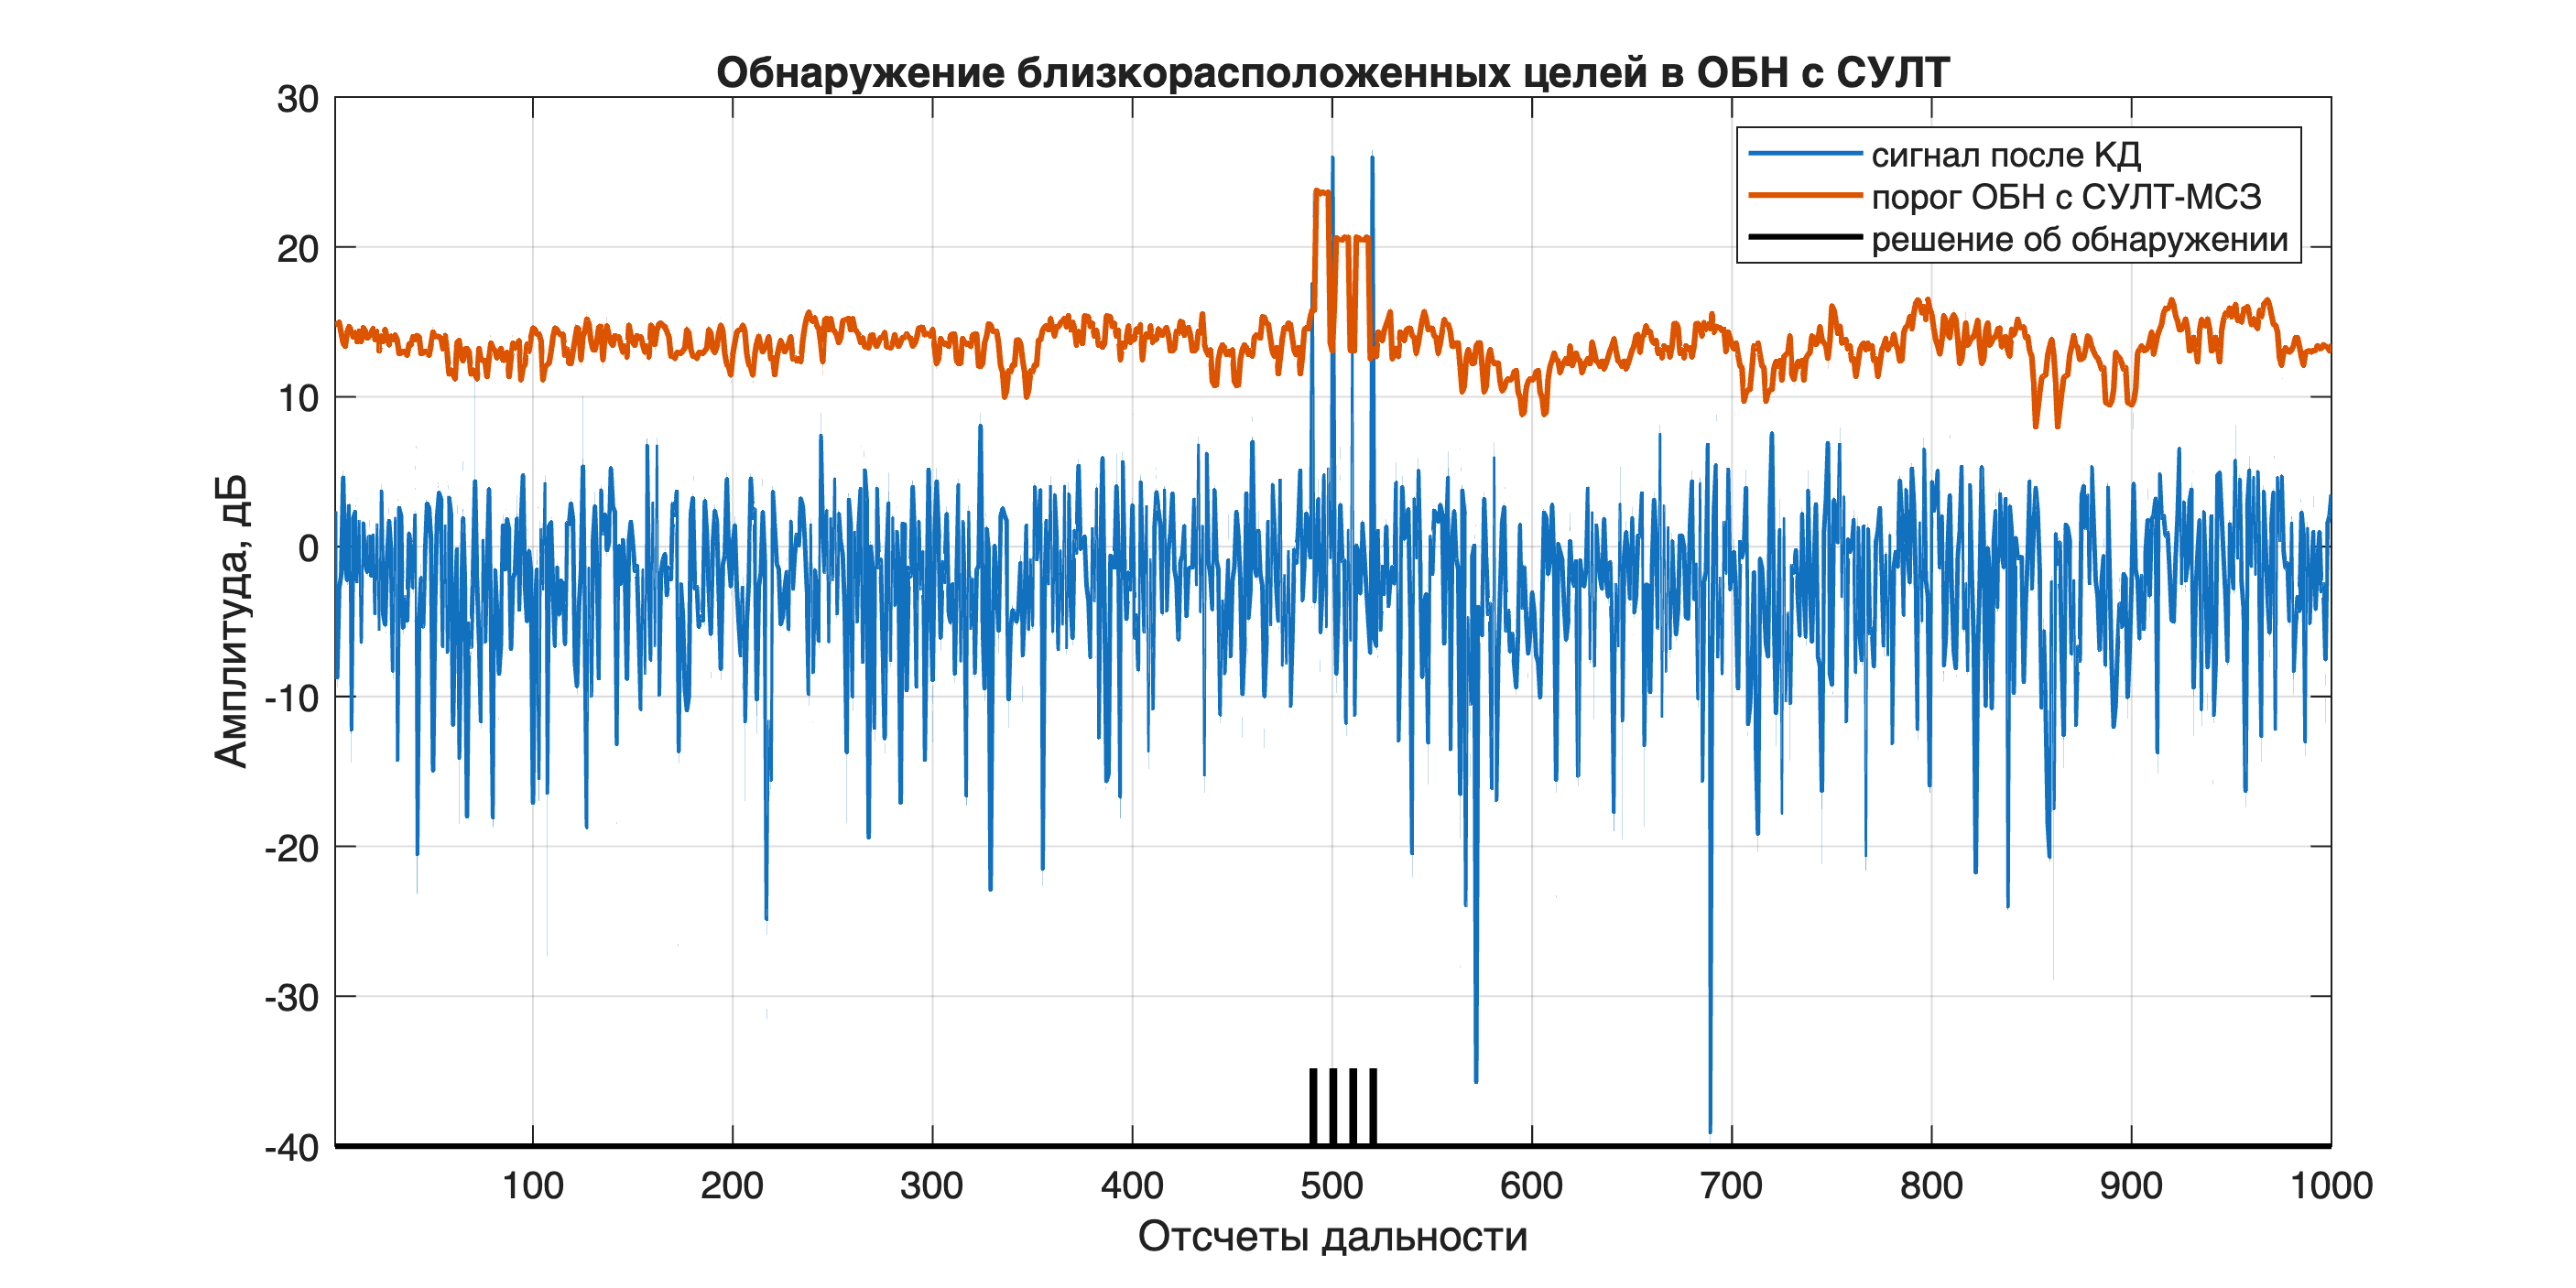
\includegraphics[width=0.85\textwidth]{export_figs/fig_hmte_tb.png}
    \caption{Обнаружение близкорасположенных целей в ОБН с СУЛТ-МСЗ}
    \label{fig:hmte_tb}
\end{figure}

Из графика видно, что все четыре близкорасположенные цели успешно обнаружены (четыре вертикальных маркера в интервале $490\dots520$ отсчетов). При попадании мешающих эхо-сигналов в одну из половин скользящего окна (длиной $N/2 = 8$ ячеек) вторая половина остается свободной от сигналов соседних целей. Алгоритм МСЗ выбирает минимальное из двух средних значений, благодаря чему оценка фонового шума не искажается и эффект взаимомаскирования устраняется. Скачки порога до уровня $21\dots24\text{ дБ}$ возникают только на тех участках, где мешающие цели одновременно присутствуют в обеих половинах скользящего окна, что не затрагивает сами отсчеты расположения целей.

\subsection{Зависимость вероятности ложной тревоги от порогового множителя в гомогенных условиях}

На четвертом этапе исследована зависимость вероятности ложной тревоги $P_{\text{лт}}$ от величины порогового множителя $\alpha$ в гомогенных условиях работы путем аналитического расчета и статистического моделирования методом Монте-Карло ($10^6$ испытаний). Результат представлен на рисунке~\ref{fig:he_pfa}.

\begin{figure}[H]
    \centering
    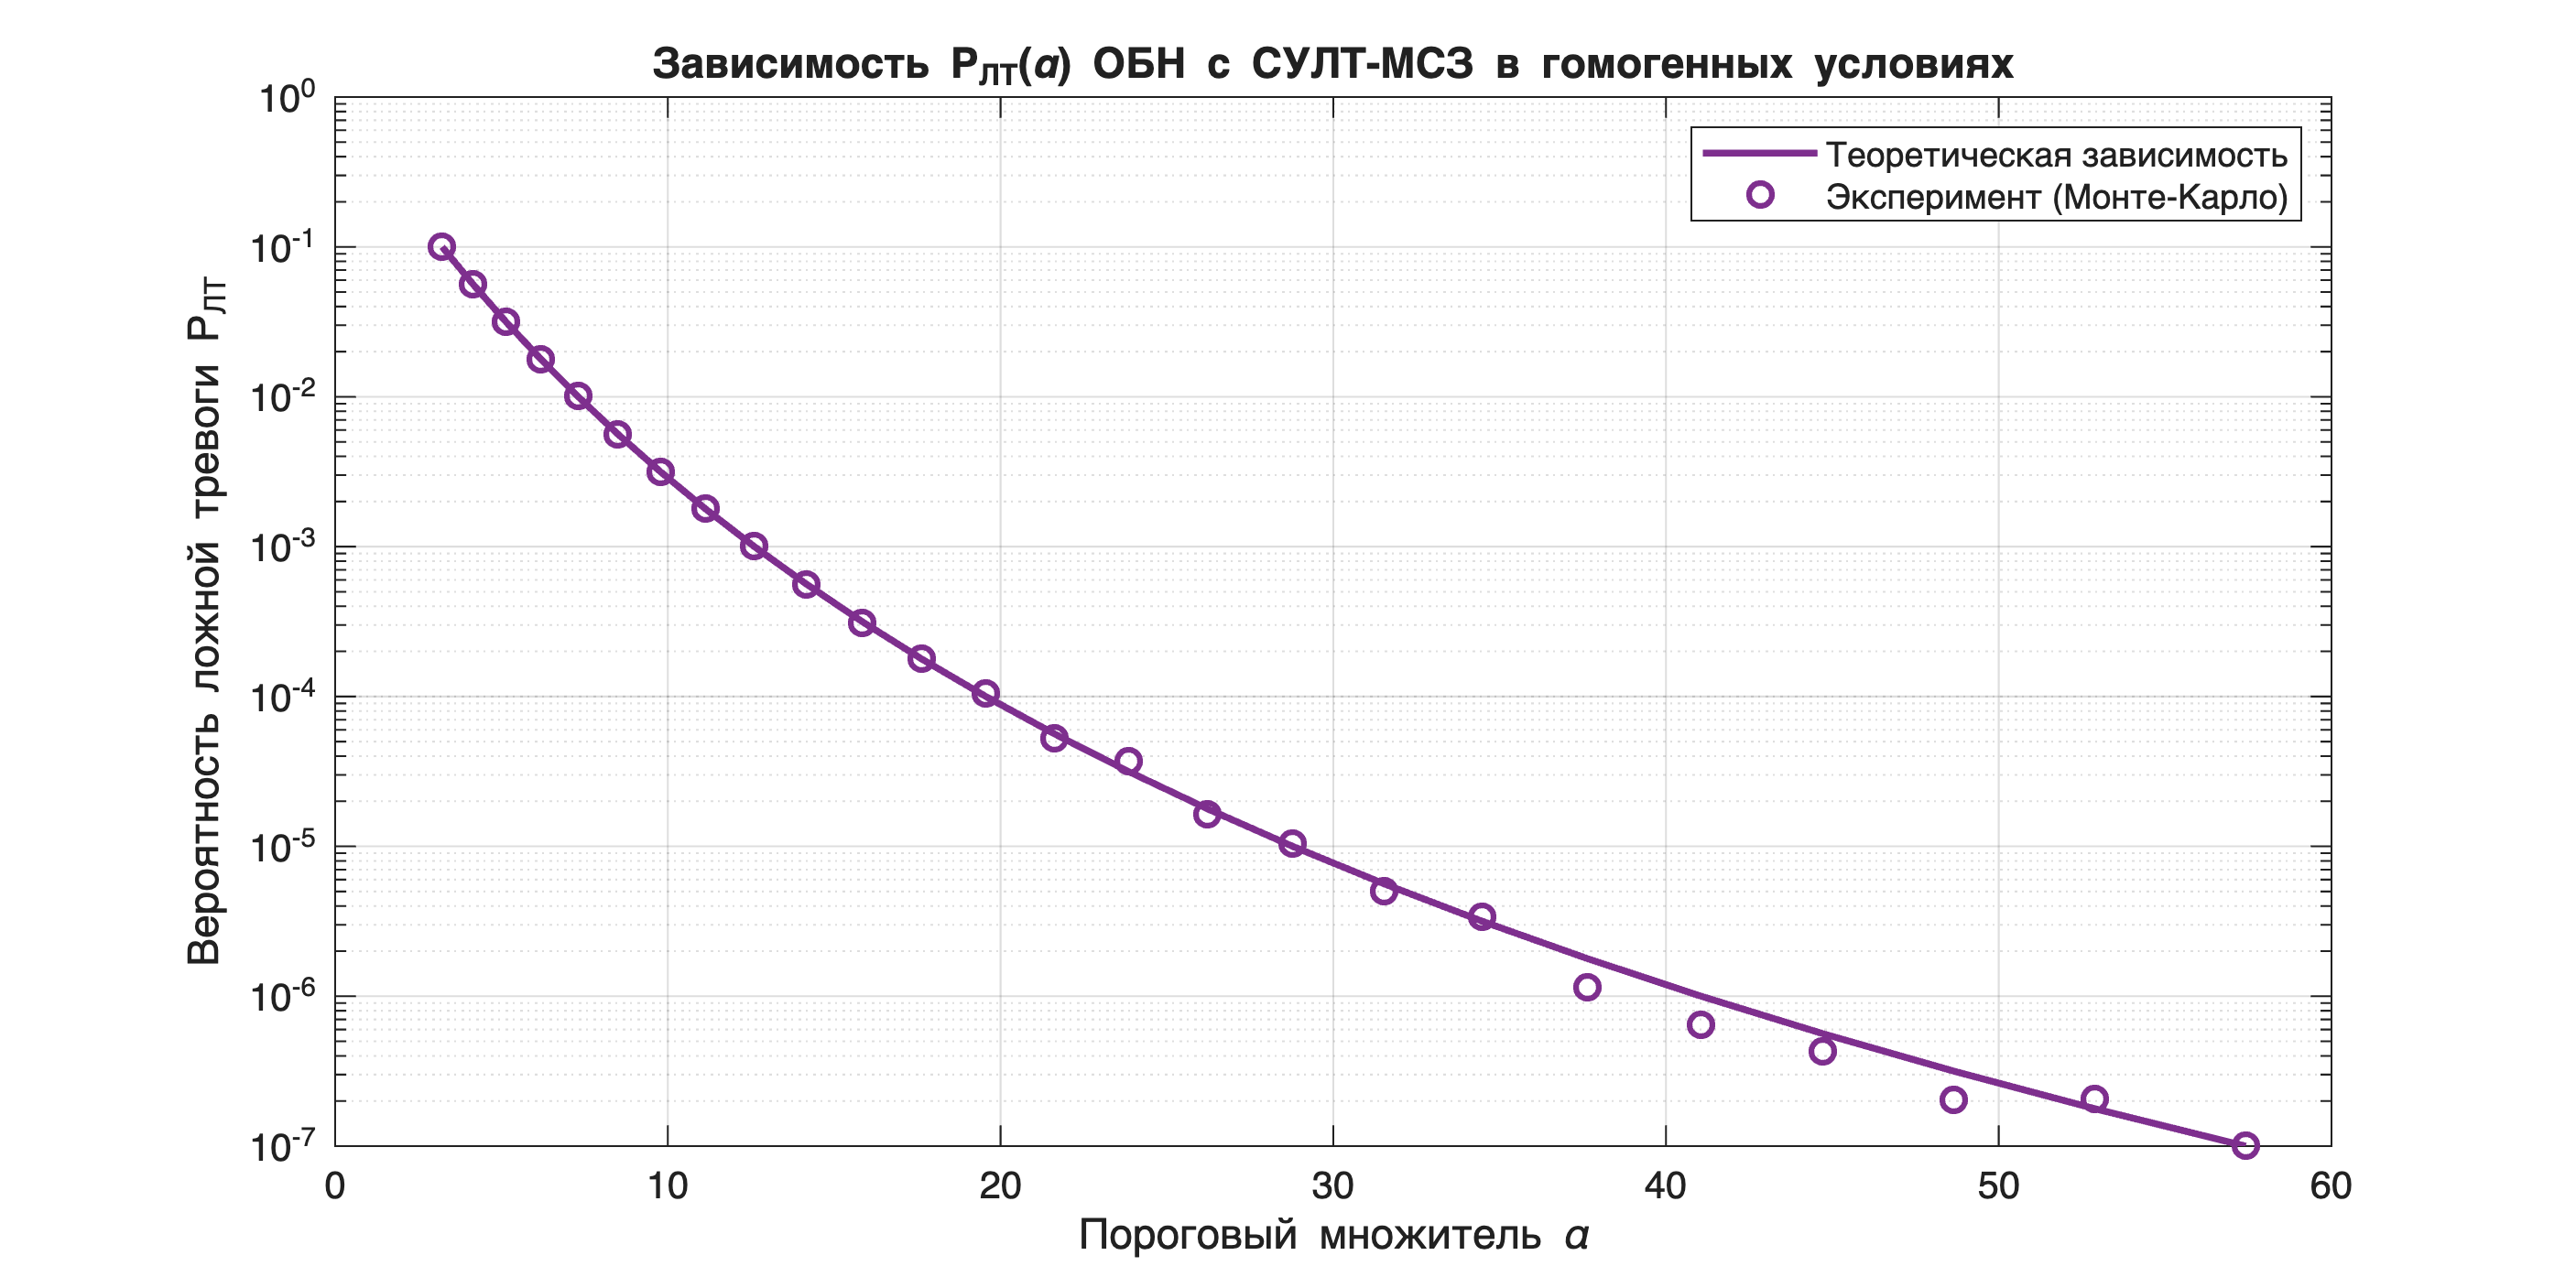
\includegraphics[width=0.85\textwidth]{export_figs/fig_he_pfa.png}
    \caption{Зависимость вероятности ложной тревоги $P_{\text{лт}}(\alpha)$ ОБН с СУЛТ-МСЗ в гомогенных условиях}
    \label{fig:he_pfa}
\end{figure}

Из графика видно, что с ростом порогового множителя $\alpha$ вероятность ложной тревоги монотонно убывает по закону, близкому к экспоненциальному. Экспериментальные точки статистического моделирования полностью согласуются с теоретической кривой (незначительный разброс в области $P_{\text{лт}} \le 10^{-6}$ обусловлен ограниченным объемом выборки испытаний $10^6$). Для заданного по варианту уровня $P_{\text{лт}} = 10^{-5}$ при длине окна $N = 16$ требуемое значение порогового множителя составляет $\alpha_{\text{МСЗ}} = 28.78$.

\subsection{Зависимость вероятности ложной тревоги на границе помех}

На пятом этапе исследовано изменение вероятности ложной тревоги $P_{\text{лт}}$ при прохождении скользящего окна обнаружителя через ступенчатую границу помех с перепадами мощности $\text{ОПШ} = 15\text{ дБ}$ и $\text{ОПШ} = 35\text{ дБ}$. Результат моделирования представлен на рисунке~\ref{fig:cwe_pfa}.

\begin{figure}[H]
    \centering
    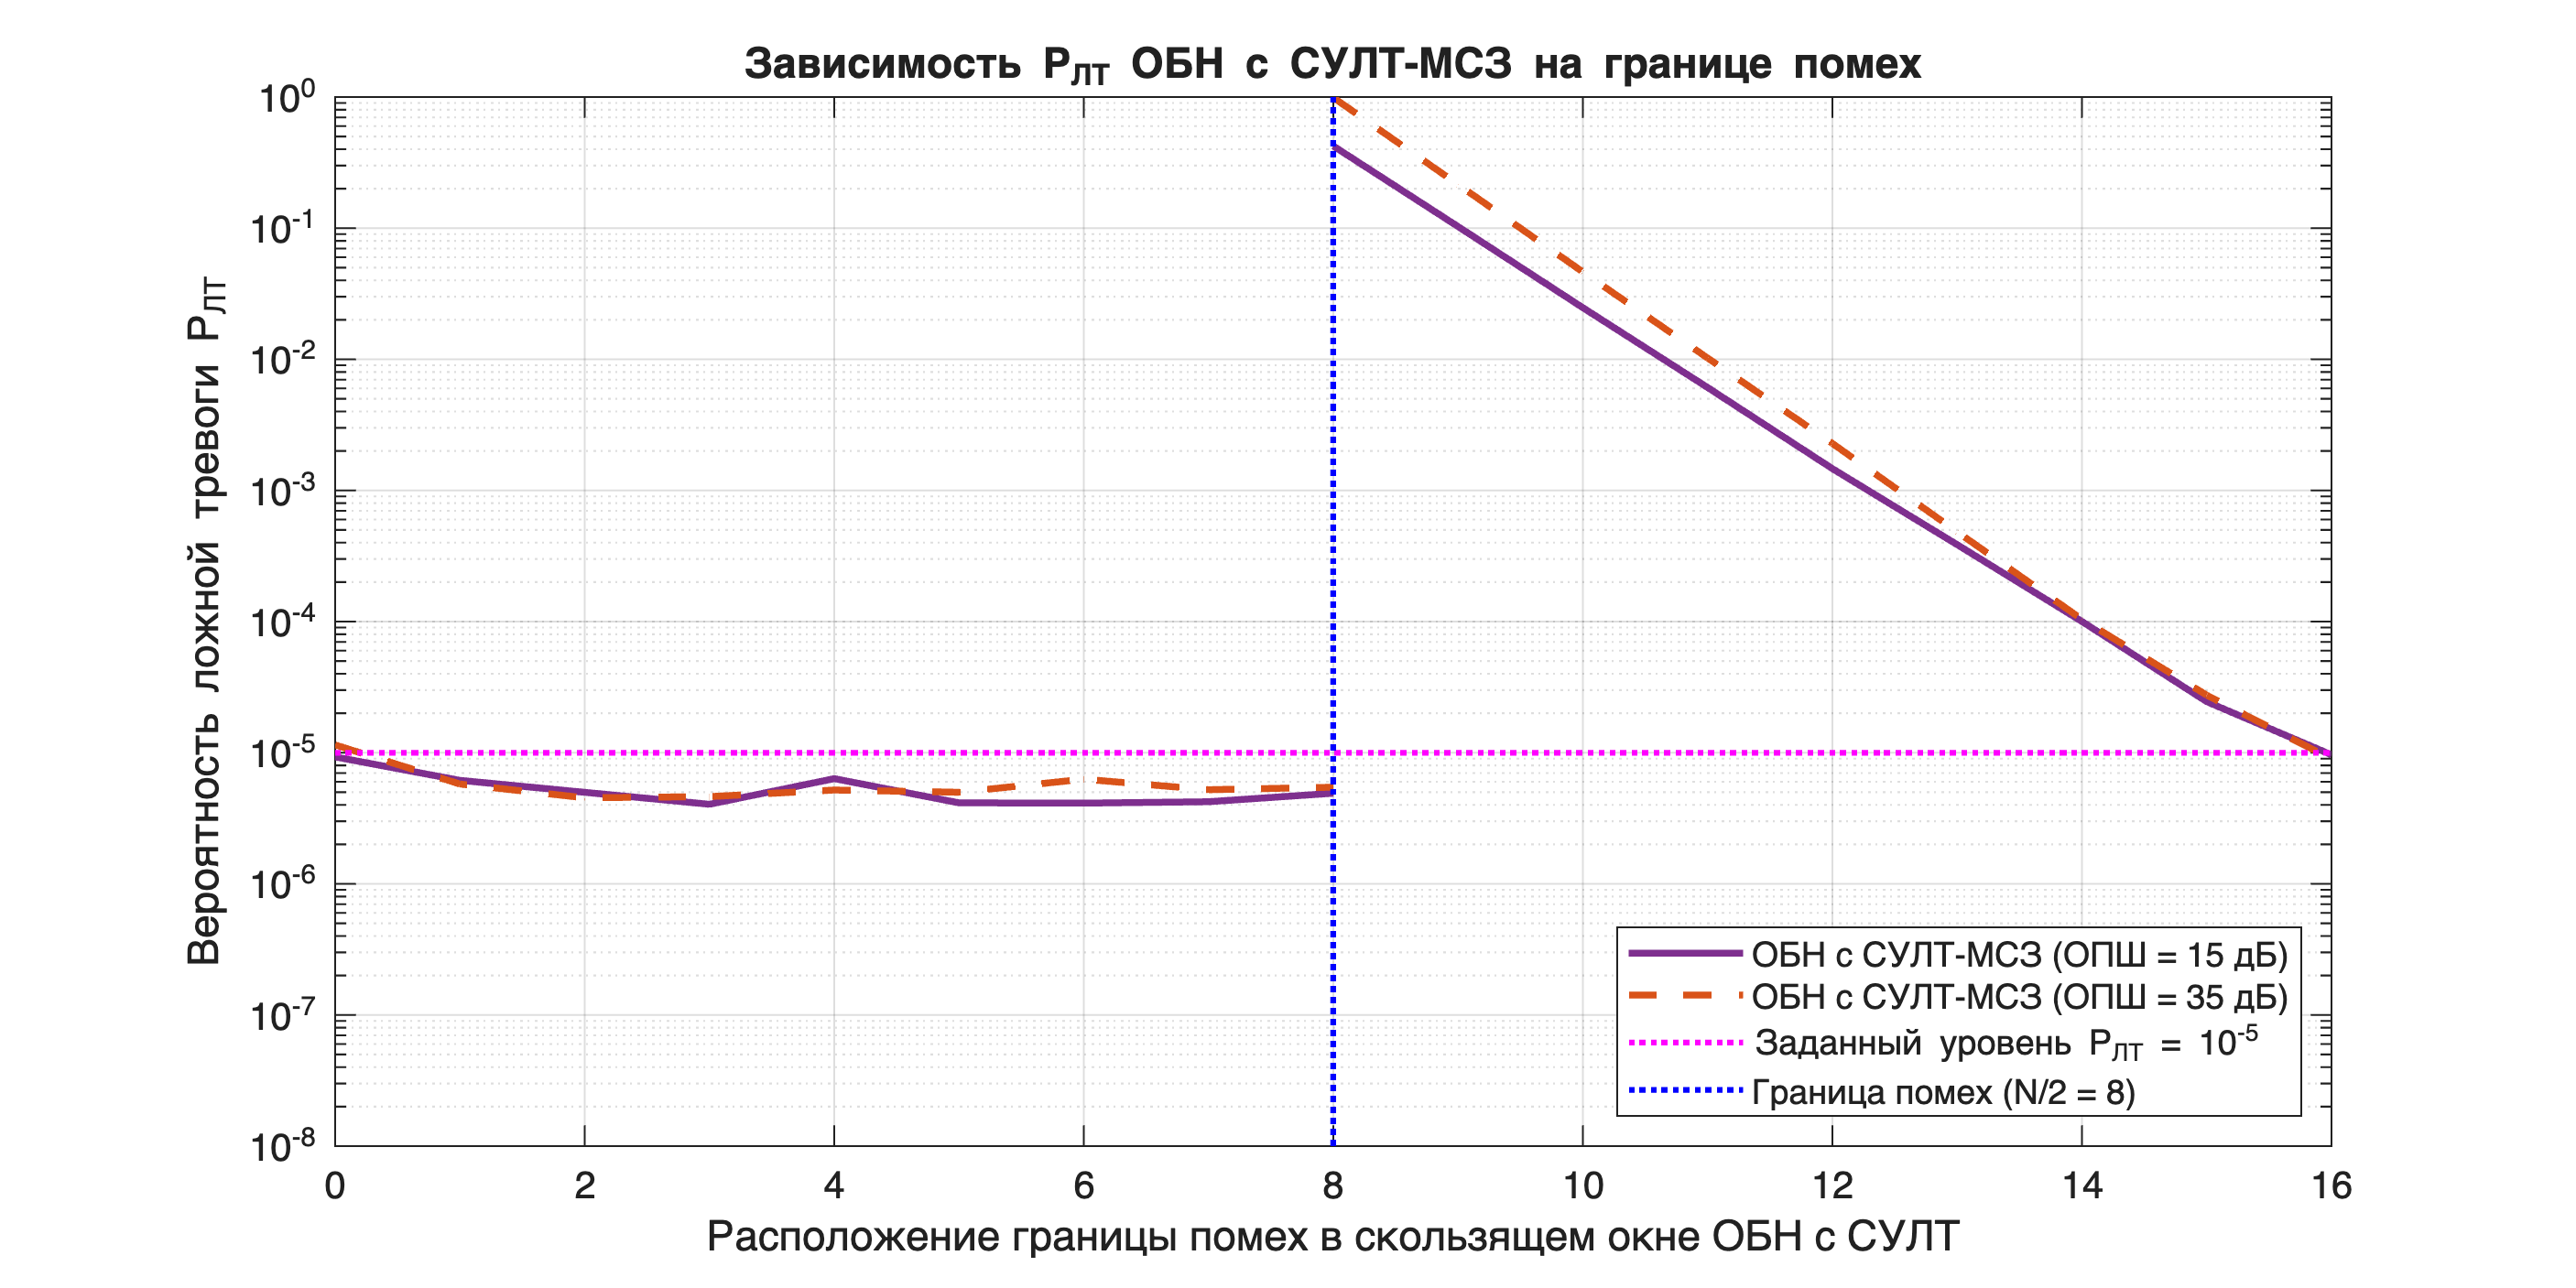
\includegraphics[width=0.85\textwidth]{export_figs/fig_cwe_pfa.png}
    \caption{Зависимость вероятности ложной тревоги $P_{\text{лт}}$ ОБН с СУЛТ-МСЗ на границе помех}
    \label{fig:cwe_pfa}
\end{figure}

Анализ кривых показывает принципиальную асимметрию поведения алгоритма МСЗ относительно центральной точки окна ($N/2 = 8$). Пока тестируемый отсчет находится в области слабого собственного шума (число ячеек с помехой от $0$ до $7$), одно из полуокон остается полностью свободным от интенсивной помехи. Благодаря выбору меньшего среднего значения порог не завышается, и фактическая $P_{\text{лт}}$ стабильно удерживается в пределах $(4\dots6)\cdot 10^{-6}$ независимо от величины ОПШ. Однако в момент перехода тестируемого отсчета через границу в область интенсивной помехи (начиная с $8$-й позиции) отстающая половина окна все еще заполнена слабым шумом. Выбор минимальной оценки приводит к сильному занижению порога и скачкообразному росту вероятности ложной тревоги до $P_{\text{лт}} \approx 0.41$ при $\text{ОПШ} = 15\text{ дБ}$ и $P_{\text{лт}} \approx 0.96$ при $\text{ОПШ} = 35\text{ дБ}$. По мере дальнейшего продвижения окна ($8 \to 16$) и заполнения отстающей части помехой $P_{\text{лт}}$ монотонно снижается до номинального значения $10^{-5}$.

\subsection{Зависимость вероятности правильного обнаружения на границе помех}

На шестом этапе исследована зависимость вероятности правильного обнаружения $P_{\text{по}}$ цели с фиксированным $\text{ОСШ} = 20\text{ дБ}$ при прохождении скользящего окна через ступенчатую границу помех с уровнями $\text{ОПШ} = 15\text{ дБ}$ и $\text{ОПШ} = 35\text{ дБ}$. Результат моделирования представлен на рисунке~\ref{fig:cwe_pd}.

\begin{figure}[H]
    \centering
    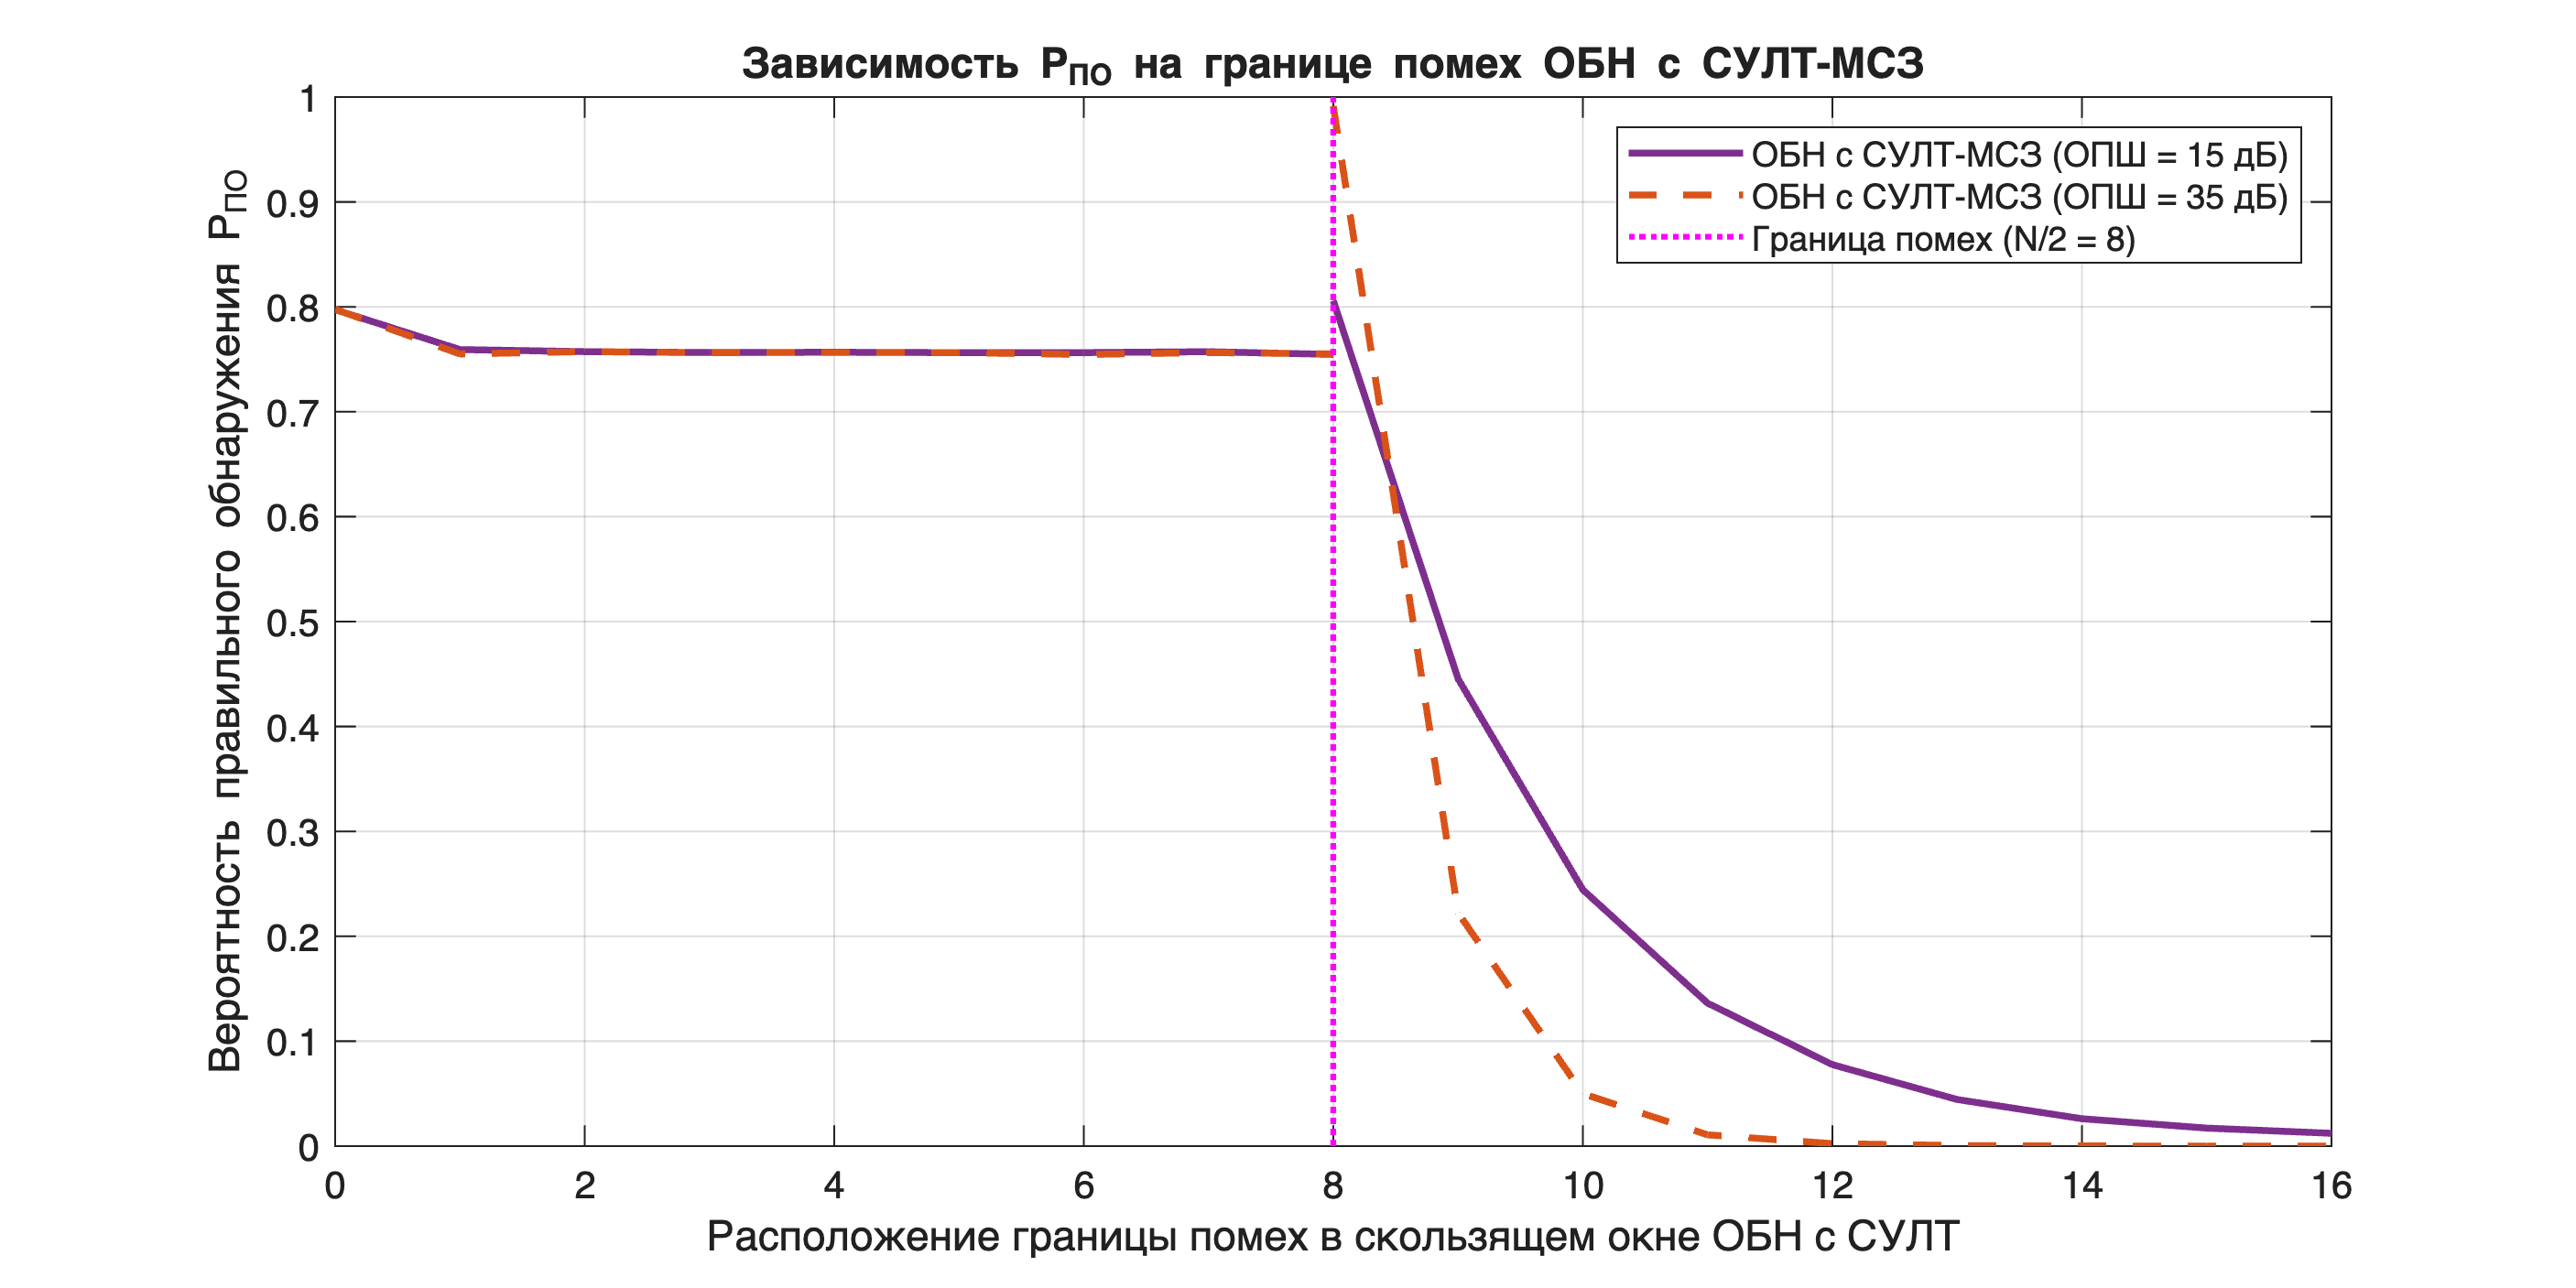
\includegraphics[width=0.85\textwidth]{export_figs/fig_cwe_pd.png}
    \caption{Зависимость вероятности правильного обнаружения $P_{\text{по}}$ на границе помех ОБН с СУЛТ-МСЗ}
    \label{fig:cwe_pd}
\end{figure}

Из графика видно, что до пересечения границы помех ($0 \le M_{\text{Б}} < 8$), когда тестируемый отсчет находится в области собственного шума, алгоритм МСЗ эффективно предотвращает маскирование цели помехой из соседнего полуокна: вероятность правильного обнаружения стабильно сохраняется на уровне $P_{\text{по}} \approx 0.76\dots0.80$ для обоих значений ОПШ. В момент перехода границы ($M_{\text{Б}} = 8$) за счет занижения порога по слабошумовой половине окна наблюдается кратковременный скачок $P_{\text{по}}$ (до $0.80$ при $\text{ОПШ} = 15\text{ дБ}$ и до $0.99$ при $\text{ОПШ} = 35\text{ дБ}$). При дальнейшем заполнении отстающей части окна интенсивной помехой ($M_{\text{Б}} > 8$) порог возрастает пропорционально мощности помехи, и вероятность обнаружения цели с $\text{ОСШ} = 20\text{ дБ}$ резко падает (практически до нуля при $\text{ОПШ} = 35\text{ дБ}$ и до $\approx 0.01$ при $\text{ОПШ} = 15\text{ дБ}$).

\subsection{Зависимость вероятности правильного обнаружения и потерь при наличии близкорасположенных целей}

На заключительном этапе исследованы характеристики обнаружения (вероятность правильного обнаружения $P_{\text{по}}$ и потери на обнаружение $L$) в гетерогенных условиях при наличии $N_M = 3$ близкорасположенных мешающих целей в одной из половин скользящего окна. Результаты моделирования представлены на рисунках~\ref{fig:hmte_pd} и~\ref{fig:hmte_loss}.

\begin{figure}[H]
    \centering
    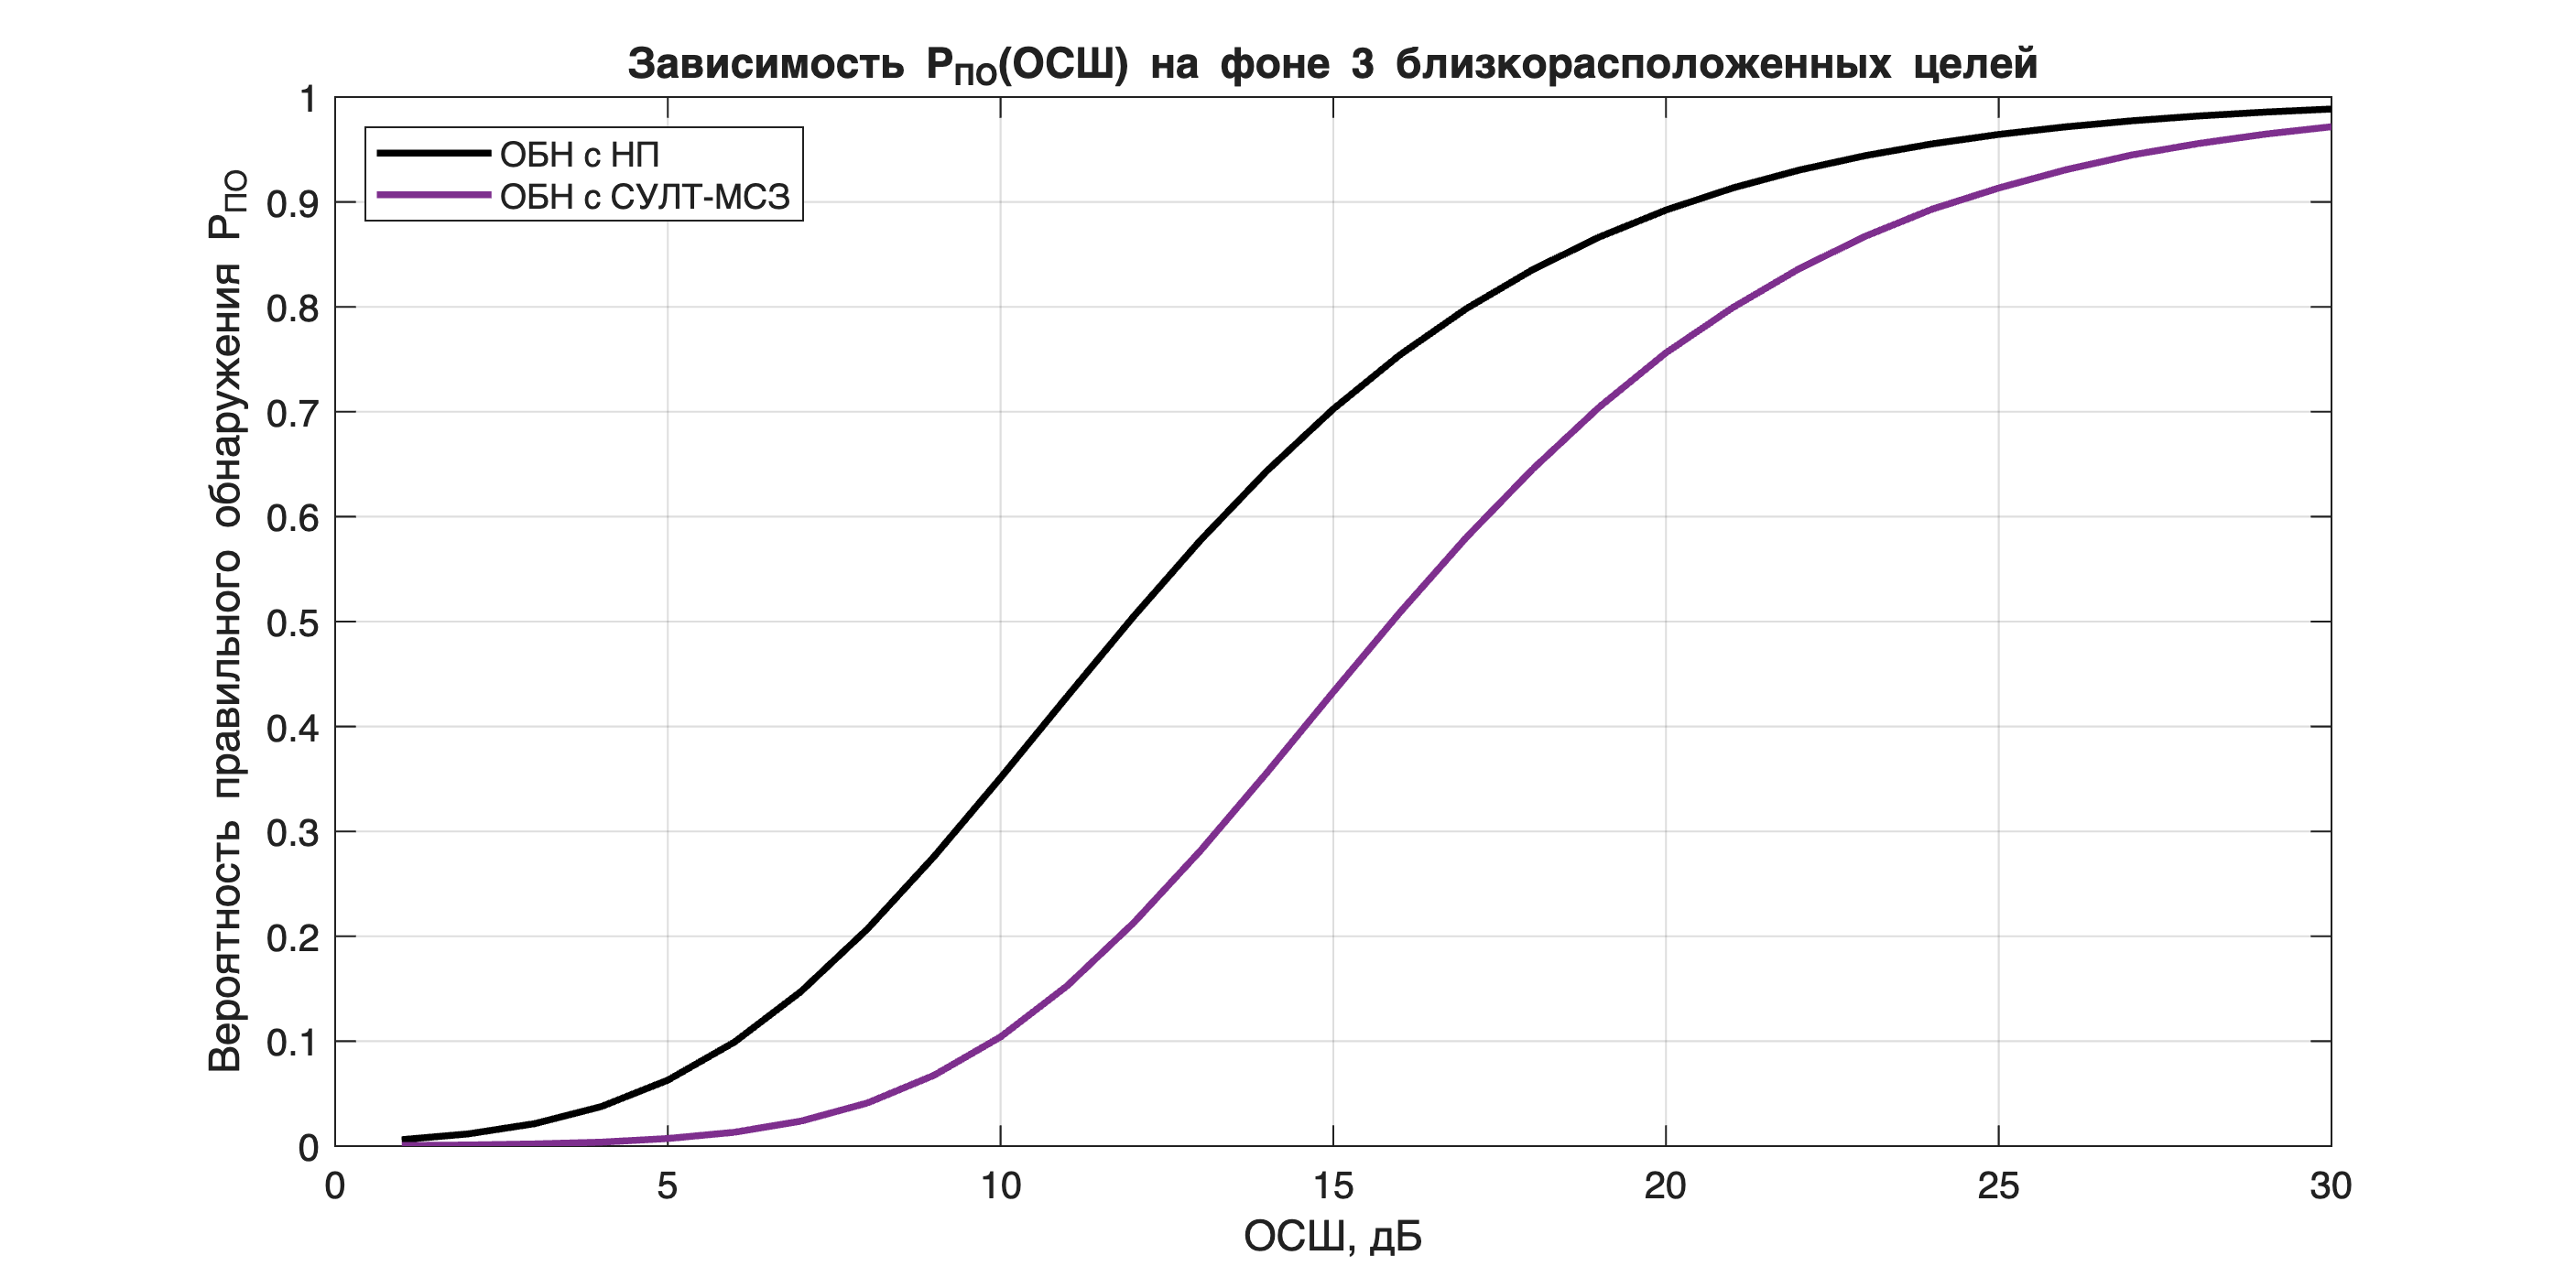
\includegraphics[width=0.85\textwidth]{export_figs/fig_hmte_pd.png}
    \caption{Зависимость вероятности правильного обнаружения $P_{\text{по}}(\text{ОСШ})$ на фоне $3$ близкорасположенных целей}
    \label{fig:hmte_pd}
\end{figure}

\begin{figure}[H]
    \centering
    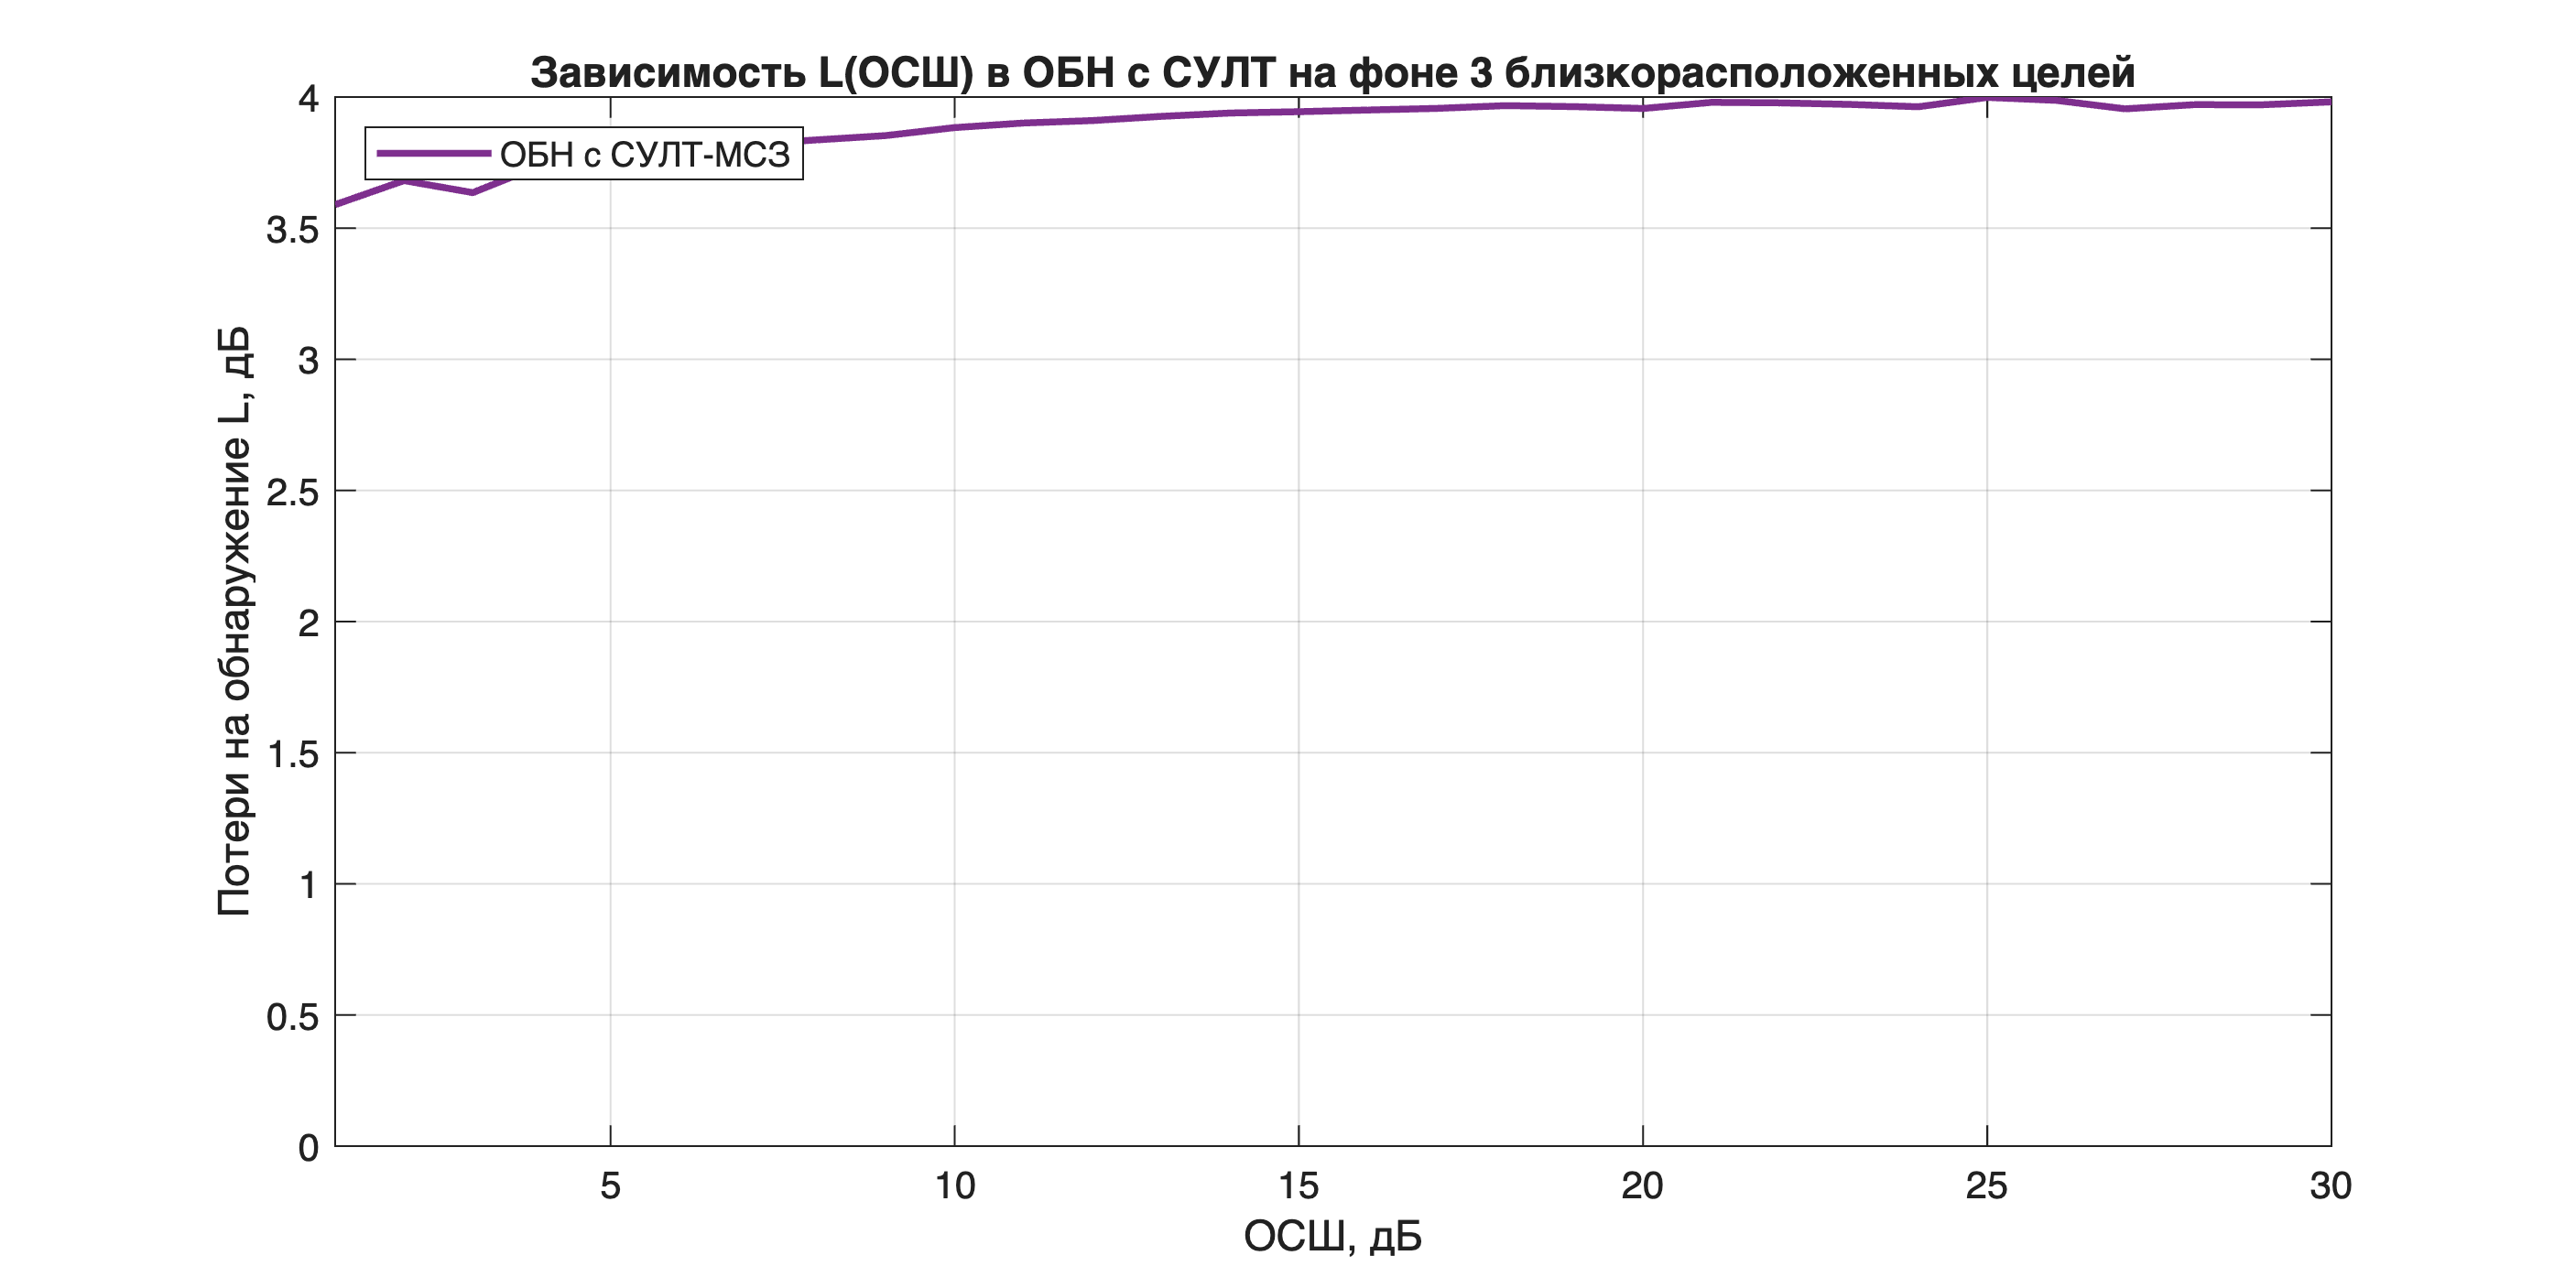
\includegraphics[width=0.85\textwidth]{export_figs/fig_hmte_loss.png}
    \caption{Зависимость потерь на обнаружение $L(\text{ОСШ})$ в ОБН с СУЛТ-МСЗ на фоне $3$ близкорасположенных целей}
    \label{fig:hmte_loss}
\end{figure}

Из представленных зависимостей видно, что при расположении всех $N_M = 3$ мешающих целей в одной из половин окна (длиной $N/2 = 8$ ячеек) обнаружитель с СУЛТ-МСЗ сохраняет работоспособность без эффекта насыщения (взаимомаскирования): при заданном по варианту значении $\text{ОСШ} = 20\text{ дБ}$ вероятность правильного обнаружения достигает $P_{\text{по}} = 0.7563$ (для оптимального обнаружителя Неймана--Пирсона с априорно известной мощностью шума $P_{\text{по}} \approx 0.893$). Потери на обнаружение $L$ по сравнению с обнаружителем Неймана--Пирсона во всем диапазоне $\text{ОСШ} \ge 10\text{ дБ}$ остаются практически постоянными и составляют около $3.9\dots4.0\text{ дБ}$ ($L = 3.96\text{ дБ}$ при $\text{ОСШ} = 20\text{ дБ}$), что обусловлено сокращением эффективного объема обучающей выборки до $N/2 = 8$ ячеек и статистикой выбора минимума.
